\chapter{Introducción}\label{chap:intro}

    \par  La cantidad de alumnos del \acrfull{dcc}, ha aumentado considerablemente en los últimos 5 años\footnote{Este aumento se ve en la recopilación de los claustros de padrones para las votaciones del \acrshort{cadcc} y en datos obtenidos de los titulados desde ucampus \cite{CADCC2002}, \cite{CADCC2016}, \cite{CADCC2018}, \cite{CADCC2021}, \cite{CADCC2022}}. Pasamos de aproximadamente 300 alumnos a más de 500 en pocos años (ver figura \ref{fig:aumento_alumnos}). En el caso de los titulados pasamos de 13 en 2012 a más de 50 en 2021, y contando los alumnos en vías de titulación estos ascendían a 61 el 2022. Este aumento estudiantil viene acompañado de una serie de desafíos, no solo en la docencia, sino en los procesos administrativos, tanto para funcionarios como profesores.

    \begin{figure}[h]
        \centering
        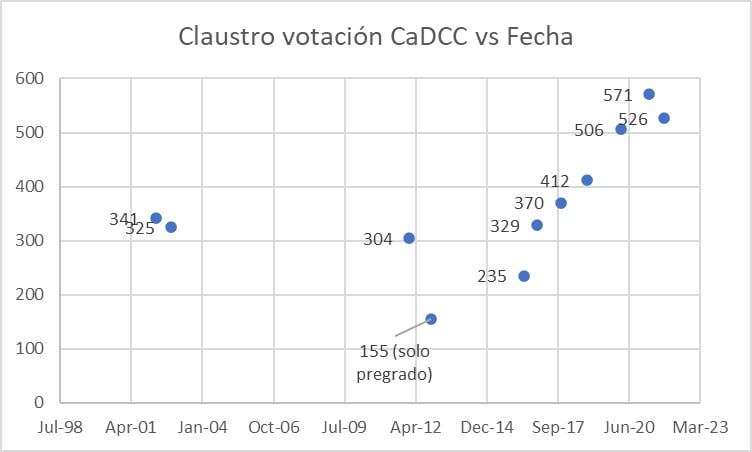
\includegraphics[scale=0.6]{media/imagenes/claustro_votacion_cadcc.jpg}
        \caption[Claustro votaciones \acrshort{cadcc}]{Claustro de las votaciones cadcc desde el 2002 hasta la fecha.}
        \label{fig:aumento_alumnos}
    \end{figure}

\section{Contexto}\label{sec:intro-con}
    \par Uno de los focos de estos desafíos son los procesos de titulación \cite{ARANCIBIA2021}. Asociados a ellos, encontramos informes con reglas de formato, un tipo específico de contenido, procedimientos, pagos, regularizaciones, que junto a otros elementos causan incertidumbre a los alumnos. En relación con ellos, hay varias fuentes de información que atañen a diversos aspectos de estos trabajos, como la wiki de titulación, las páginas del centro de alumnos, publicaciones oficiales en U-Cursos, etc. A pesar de tener estos recursos disponibles, muchas veces, la mayoría de los estudiantes suele preguntar directamente a sus profesores y, funcionarios como la secretaria del departamento suelen recibir la mayor cantidad de dudas no resueltas \cite{ARANCIBIA2021}.
    
    \par Una de las soluciones a considerar, podría ser ampliar personal, lo cual debe ser debidamente justificado, y consensuado \cite{Chile2014}. Por otra parte, tampoco es lo que buscan los estudiantes, pues a la mayoría le gustaría un acceso directo a la información sin pasar por intermediarios \cite{ARANCIBIA2021}. Y es justamente en este ambiente, que el proyecto Mesa de Ayuda Virtual, se posiciona como una buena alternativa para asistir a los estudiantes.
    
    \par El proyecto Mesa de Ayuda Virtual, es un proyecto de soporte o asistencia digital, iniciado por Pablo Arancibia Barahona (egresado del DCC), que busca responder a la necesidad de mejorar el proceso de titulación de alumnos(as). Actualmente está dividido en dos áreas: La primera es un \textit{bot} de \textit{Telegram}, con funcionalidades como preguntas frecuentes agrupadas por proceso, capacidad de feedback por parte del usuario y contactar a un asistente. La segunda, es una página web, que cuenta con un \textit{front-end} para alumnos y otro para administradores, en ellos se puede categorizar preguntas, acceder y modificar los procesos vigentes con sus preguntas, dispone de chat directo con los estudiantes (que usen el bot), entre otros.
    
    \par Este proyecto responde a las necesidades del estudiantado, pues fue diseñado a partir de la información levantada en el departamento y la consideración de las necesidades allí expuestas. Fue validado por la docencia y el centro de estudiantes y, ha finalizado su primera etapa de desarrollo. Actualmente, soporta más procesos como prácticas profesionales.

    \begin{figure}[h]
        \centering
        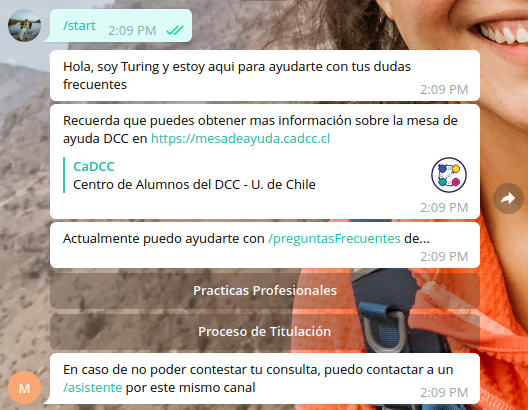
\includegraphics[scale=0.3]{media/imagenes/sc/inicio_bot.png}
        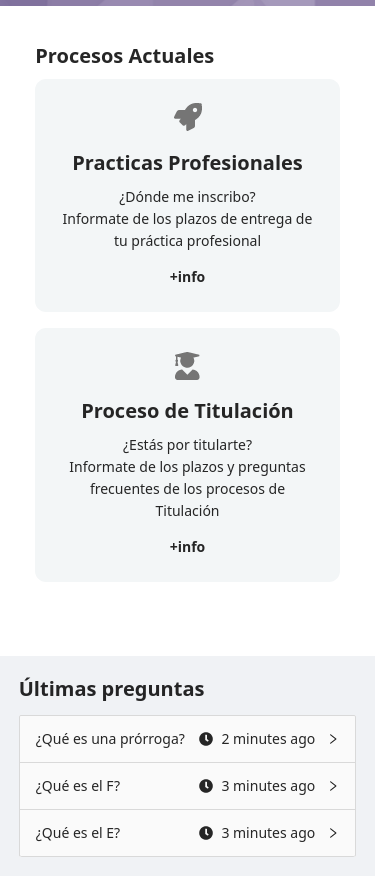
\includegraphics[scale=0.3]{media/imagenes/sc/mesa-de-ayuda-front-mobile-recorte.png}
        \caption[Vista inicio del \textit{bot} y página web]{Imágenes de vista de inicio del \textit{bot} y de la página web de la mesa de ayuda.}
        \label{fig:home-img-bot}
    \end{figure}

\section{Problema}\label{sec:intro-pro}
    \par Como se habló anteriormente, la solución consta de dos partes vitales la web y el \textit{bot}. Dentro de las conclusiones más relevantes del trabajo de Arancibia, destaca el hecho de que la mayoría de los encuestados, dijo que optaría por usar el servicio del \textit{bot} de \textit{Telegram}. Sin embargo, este proyecto no está implementado y presenta algunas falencias en su desarrollo que impiden hacerlo extensible, principalmente en el código del bot. En ese sentido, el que una parte vital del proyecto no pueda tener soporte es algo crítico. 
    \par Además la ausencia de personalización, en un sistema de información, podría hacer que los usuarios lo dejen de usar, ya que este es un factor clave en un sistema como este \cite{Paz2021}.
    \par El presente trabajo busca aportar en la continuidad del proyecto, enfocándose en resolver los problemas descritos en los objetivos.

\section{Objetivos}\label{sec:intro-obj}
  \subsection*{Objetivo General}\label{sec:obj-g}
       El objetivo general es extender el sistema actual, agregando funcionalidades que permitan crear un sistema extensible, personalizado y confiable. El cual será actualizado principalmente por el \acrshort{cadcc}, con miras de integrar otros actores posteriormente, favoreciendo la continuidad de este servicio.
        
    \subsection*{Objetivos Específicos}\label{sec:obj-e}
        \begin{enumerate}
            \item Analizar la solución existente, con el fin de identificar qué modificaciones son relevantes, tanto para que el modelo de datos soporte las nuevas funcionalidades, como para saber la manera en que se debe reestructurar el código.
            
            \item Rediseñar los modelos y funcionalidades, para que el sistema acepte las modificaciones necesarias.
            
            \item Diseñar nuevos componentes de confiabilidad que permitan añadir información a las respuestas y mejorar el modelo de feedback del usuario, para que se pueda obtener más información como su vigencia.
            
            \item Diseñar un modelo de subscripción personalizada: que contempla una búsqueda personalizada de procesos, un elemento suscriptor, variables relevantes de notificar y un modelo de notificaciones y data del alumno, entre otras \textit{features} relevantes para los alumnos.
            
            \item Implementar y probar las reestructuraciones, asegurando la integridad del modelo de datos, del código y permitiendo su extensibilidad a través de la modularidad lógica.
            
            \item Implementar y probar las nuevas funcionalidades buscando que sean aquellas relevantes para los alumnos.
        \end{enumerate}
         
    \subsection*{Evaluación}\label{sec:eval}
    Para validar que el objetivo se cumplió, hay dos áreas que tomar en cuenta: La integridad del sistema y la validez de las nuevas funcionalidades.
    \par En relación con la primera, se espera que las modificaciones hechas le permitan al sistema seguir cumpliendo con sus objetivos. Para lo cual se creará y usará una serie de tests que permitan asegurar sus funcionalidades críticas y la integridad del sistema. Por ejemplo, en el \textit{back-end} probando los \textit{end-points}, que los modelos permitan operaciones \textit{CRUD}, entre otros.
    
    \par En relación con la validez de las nuevas funcionalidades, se propone hacer tests de usabilidad, tanto entrevistas individuales como \acrlong{f}.
    
    \par Adicionalmente, solo si es posible, se propone beta testing, porque permitiría integrar ambas áreas y acercar el producto al usuario. Pero esto depende de la disponibilidad del \acrshort{cadcc}, así como de que el sistema ya esté desplegado por ellos.

\section{Solución Propuesta}\label{sec:intro-sol}
    \par Para poder llevar a cabo los objetivos anteriormente descritos, se propone agruparlos en 3 fases: Análisis, Diseño e Implementación. Pensadas en la lógica que abarca cada uno de estos objetivos.
    
    % Modificaciones
    \par El Análisis tiene el propósito de asegurar la mantenibilidad y rescatar las funcionalidades críticas. Para lo cual, se estudiará en detalle la solución actual. Con esto se busca identificar todos aquellos aspectos relevantes, así como aquellos que necesiten una modificación, ya sea una reestructuración o reimplementación. Entre ellos: las modificaciones en el modelo de datos, las refactorizaciones en el código para modularizar la solución actual y darle una estructura lógica, que permitan entender el sistema y hacerlo extensible.
    
    \par A partir de este proceso, se diseñarán y usarán tests que sirvan para validar como el sistema actual responde a los objetivos originales y los planteados en esta propuesta. Luego con el conjunto de test diseñados, cuando existan modificaciones, se probará que no afectaron la funcionalidad original ya implementada.
    
    % Features de confiabilidad
    \par Durante el Diseño,  se buscará agregar elementos de confiabilidad y generar un modelo de subscripción.
    
    \par Para mejorar la confiabilidad se agregará a las respuestas, la fuente de la información y su última actualización. Y junto con esto, la capacidad del usuario de retroalimentar al sistema, permitiendo ayudar a establecer métricas de vigencia reales, basadas en las calificaciones de los usuarios, así como proporcionar ayuda a los administradores del sistema, al poner atención a aquellos procesos que requieren realmente una actualización, lo que permite enfocar los esfuerzos.
    
    \par Se creará un modelo de subscripción, este permitirá buscar y seleccionar un proceso de forma individual, por ejemplo: \guillemotleft El proceso de titulación otoño 2022\guillemotright.  A partir de esta búsqueda, se debe permitir suscribirse no solo al proceso global, sino que de forma más específica a información que sea relevante para el alumno, por ejemplo: fechas de entrega, requisitos, consecuencias, entre otros\footnote{A estos elementos se les denominó \guillemotleft elemento subscriptor\guillemotright en los objetivos.}.
    
    \par Así mismo, hay que generar un modelo de notificaciones, que se ajuste a estas necesidades, y que sea lo suficientemente simple como para poder extenderlo sin problemas.
   
    \par Al final de esta fase, se debe validar estos modelo con usuarios, y entidades relevantes para hacer un ajuste, antes de comenzar con la etapa de implementación. Estas validaciones deben contemplar todos los aspectos ya mencionados como nuevas funcionalidades, centrándose en la relevancia de cada una para del estudiante. Al mismo tiempo, el agregar nuevas funcionalidades y personalización que dependa de datos del usuario, puede levantar problemas de privacidad que deben ser revisados junto a los encuestados.
    % Implementación

    \par La última fase es la implementación de las funcionalidades ya validadas. Este proceso busca integrar estas funcionalidades, tanto al \textit{back-end} como al \textit{front-end}. Por lo tanto, nuevamente se requerirá de un alto grado de cuidado para no romper las funcionalidades ya implementadas.
    % Validación
    \par Estas \textit{features} deben ser testeadas. Además se incluirá un proceso de validación con los usuarios que incluya demos. Opcionalmente, pero no depende del memorista, se plantea la posibilidad de incluir estas funcionalidades en un sistema de producción. Pero esto depende del \acrshort{cadcc} y de la disponibilidad de sus miembros.
    % Documentación y extras.
    \subsection{Documentación}
    \par Aunque la documentación no representa un desafío técnico elevado, se quiere destacar su rol, en la extensibilidad de un sistema, por lo que, se requiere tiempo, especial en cada iteración, para realizar una buena documentación del sistema.
    % Dentro de otros aspectos no fundamentales este sistema incluirá una forma de auditar el tiempo de respuesta, las fuentes de información confiable, identificación y preferencias de los usuarios, así cómo métricas de uso para su mejora continua.
    
    \subsection{Tecnologías}
        Si bien la decisión de qué tecnologías usar, puede verse modificada en un futuro, según los resultados del trabajo, en primera instancia se pretende continuar con el \textit{setup} original del proyecto.\\
        Dentro de los lenguajes a utilizar se destacan: Python y JavaScript. Estos están fuertemente ligados a las herramientas que se usan en los distintos aspectos del proyecto.
        \begin{itemize}
            \item \textbf{Servidor}: El servidor funciona principalmente en \textit{\gls{Django}}, a través de la librería \textit{Django channels} se sincronizan los chats del administrador con el bot. También se pretende integrar \textit{\gls{Celery}} para el menejo de procesos asíncronos.
            \item \textbf{Motor de Base de datos:} La base de datos, inicialmente pensada para preguntas repetitivas y frecuentes, usa \textit{MongoDB}, que como herramienta \textit{NoSQL}, está especializada en este tipo de \textit{requests}. También, puede que sea necesario agregar otro tipo de motores en el transcurso del proyecto, ya que hay varias áreas sobre todo auditoría, en las que el modelo, no se ajusta completamente al enfoque \textit{NoSQL}.
            \item \textbf{Cache sesión usuario}: Se usa \textit{Redis}, para administrar las conversaciones a través de \textit{Django Channels}.
            \item \textbf{Pagina Web}: La página web, esta principalmente diseñada en \textit{React}, más algunas librerías para facilitar el desarrollo de componentes visuales. Se destaca, que idealmente esta no se encuentra en el scope del proyecto.
            \item \textbf{Telegram API}: Telegram provee de una API la opensource la que se conecta a través de websockets con el servidor.
        \end{itemize}

\section{Metodologías}\label{sec:intro-met}
    \par Para implementar lo propuesto se dividió el proyecto en 4 partes: Primero se realizó un levantamiento y análisis de datos, a partir de aquello un diseño basado en las preferencias de usuario, luego se analizó y reestructuró el código. Finalmente se realizó la implementación de las nuevas funcionalidades.

    \par Para realizar el levantamiento de información, se convocó a dos \acrlong{f}, cuyos resultados se pueden ver en la sección \ref{sec:focus}. Luego se agruparon las respuestas de los estudiantes a las diferentes materias, en áreas de interés y tópicos críticos del sistema. Después, se elaboró un análisis sobre las opiniones conjuntas de los estudiantes. Con esto se hizo una clasificación cualitativa de los estudiantes, y se resumieron sus preferencias, objetivos y funcionalidades deseadas al final de la sección correspondiente.

    \par A partir de los datos obtenidos y su análisis posterior, se generalizaron los objetivos de los estudiantes en 4 diagramas. Estos contienen sus percepciones en torno a la manera de  cumplirse esos objetivos y lo que se complementa con las funcionalidades disponibles del bot, para esquematizar la manera en que se debe realizar el desarrollo de software. Las conclusiones obtenidas en el desarrollo de este análisis permitieron hacer una implementación centrada en los objetivos del usuario.

    \par Luego se analizó en profundidad el código existente, se hicieron varias pruebas funcionales y se modificó parcialmente el código para albergar nuevas funcionalidades. A partir de este trabajo preliminar, se desarrolló una reimplementación profunda separando en capas lógicas el procesamiento de la información, lo que se dividió de las acciones que el sistema realiza a partir de las peticiones del usuario (ver sección \ref{sec:imple}).

    \par Finalmente se realizó la implementación de las nuevas funcionalidades de suscripción, se añadió documentación durante el trabajo y se realizaron una serie de correcciones de compatibilidad, para asegurar el resultado.

